\newcommand{\downloaderTagResultsAucTable}{
    \begin{table}[H]
        \centering
        \begin{tabular}{|p{2,8cm}||p{2,8cm} p{2,8cm} p{2,8cm}|}
            \hline
            Downloader Tag & ALOHA & Joint Embedding & Proposed Model \\
            \hline
            AUC-ROC & 0.973$\pm$0.003 & 0.976$\pm$0.002 & \textBF{0.980$\pm$0.000} \\
            \hline
        \end{tabular}
        \caption{AUC-ROC (Area Under Curve) of the different models for the \textbf{Downloader Tag} prediction task. Results were aggregated over \textBF{3} training runs with different weight initializations and minibatch orderings. Best results are shown in \textbf{bold}.} \label{tab:downloaderTag_auc}
    \end{table}
}

\newcommand{\downloaderTagResultsAtFprTable}{
    \begin{center}
        \begin{longtable}[c]{|p{3,2cm}||p{1,8cm} p{1,8cm} p{1,8cm} p{1,8cm} p{1,8cm}|}
            \hline
            Downloader Tag & \multicolumn{5}{c|}{{FPR}} \\
            & $10^{-5}$ & $10^{-4}$ & $10^{-3}$ & $10^{-2}$ & $10^{-1}$ \\
            \hline
            \endfirsthead

            \caption*{\raggedright ...continued from previous page} \\
            \hline
            Downloader Tag & \multicolumn{5}{c|}{\textbf{FPR}} \\
            & $10^{-5}$ & $10^{-4}$ & $10^{-3}$ & $10^{-2}$ & $10^{-1}$ \\
            \hline
            \endhead

            \caption*{\raggedleft ...continued on next page} \\
            \endfoot

            \caption{Mean and standard deviation results (TPR, Accuracy, Recall, Precision and F1-Score) of the different models for the \textbf{Downloader Tag} prediction task at different \textbf{FPR}s (\textit{False Positive Rates}). Results were aggregated over \textBF{3} training runs with different weight initializations and minibatch orderings. Best results are shown in \textbf{bold}. Under \textbf{TPR} results are also presented the percentage reduction in mean detection error and in ROC curve standard deviation introduced by the \textit{Proposed Model} with respect to both \textit{ALOHA} model and \textit{Joint Embedding}.} \label{tab:downloaderTag_results_at_fpr} \\
            \endlastfoot

            \multicolumn{6}{|c|}{\textbf{TPR}} \\
            \hline
            ALOHA & \textBF{0.227$\pm$0.103} & \textBF{0.439$\pm$0.061} & 0.550$\pm$0.045 & 0.619$\pm$0.020 & 0.942$\pm$0.002 \\
            Joint Embedding & 0.173$\pm$0.020 & 0.394$\pm$0.126 & 0.495$\pm$0.137 & 0.657$\pm$0.030 & \textBF{0.962$\pm$0.006} \\
            Proposed Model & 0.184$\pm$0.031 & 0.382$\pm$0.017 & \textBF{0.580$\pm$0.019} & \textBF{0.659$\pm$0.019} & 0.957$\pm$0.003 \\
            \hline
            Error Reduction wrt \newline ALOHA & -5.6\% & -10.2\% & 6.7\% & 10.5\% & 25.9\% \\
            Error Reduction wrt \newline Joint Embedding & 1.3\% & -2.0\% & 16.8\% & 0.6\% & -13.2\% \\
            \hline
            Std Reduction wrt \newline ALOHA & 69.9\% & 72.1\% & 57.8\% & 5.0\% & -50.0\% \\
            Std Reduction wrt \newline Joint Embedding & -55.0\% & 86.5\% & 86.1\% & 36.7\% & 50.0\% \\
            \hline
            \multicolumn{6}{|c|}{\textbf{Accuracy}} \\
            \hline
            ALOHA & \textBF{0.935$\pm$0.009} & \textBF{0.953$\pm$0.005} & 0.961$\pm$0.004 & 0.959$\pm$0.002 & 0.904$\pm$0.000 \\
            Joint Embedding & 0.931$\pm$0.002 & 0.949$\pm$0.011 & 0.957$\pm$0.011 & \textBF{0.962$\pm$0.002} & \textBF{0.905$\pm$0.000} \\
            Proposed Model & 0.932$\pm$0.003 & 0.948$\pm$0.001 & \textBF{0.964$\pm$0.002} & \textBF{0.962$\pm$0.002} & \textBF{0.905$\pm$0.000} \\
            \hline
            \multicolumn{6}{|c|}{\textbf{Recall}} \\
            \hline
            ALOHA & \textBF{0.227$\pm$0.103} & \textBF{0.439$\pm$0.061} & 0.550$\pm$0.045 & 0.619$\pm$0.020 & 0.942$\pm$0.002 \\
            Joint Embedding & 0.173$\pm$0.020 & 0.394$\pm$0.126 & 0.495$\pm$0.137 & 0.657$\pm$0.030 & \textBF{0.962$\pm$0.006} \\
            Proposed Model & 0.184$\pm$0.031 & 0.382$\pm$0.017 & \textBF{0.580$\pm$0.019} & \textBF{0.659$\pm$0.019} & 0.957$\pm$0.003 \\
            \hline
            \multicolumn{6}{|c|}{\textbf{Precision}} \\
            \hline
            ALOHA & 0.999$\pm$0.000 & \textBF{0.997$\pm$0.000} & 0.980$\pm$0.002 & 0.850$\pm$0.004 & 0.462$\pm$0.001 \\
            Joint Embedding & 0.999$\pm$0.000 & 0.997$\pm$0.001 & 0.976$\pm$0.008 & 0.857$\pm$0.006 & \textBF{0.467$\pm$0.001} \\
            Proposed Model & \textBF{1.000$\pm$0.000} & \textBF{0.997$\pm$0.000} & \textBF{0.981$\pm$0.001} & \textBF{0.857$\pm$0.004} & 0.466$\pm$0.001 \\
            \hline
            \multicolumn{6}{|c|}{\textbf{F1 Score}} \\
            \hline
            ALOHA & \textBF{0.358$\pm$0.146} & \textBF{0.607$\pm$0.061} & 0.704$\pm$0.037 & 0.716$\pm$0.014 & 0.620$\pm$0.001 \\
            Joint Embedding & 0.294$\pm$0.030 & 0.552$\pm$0.138 & 0.645$\pm$0.131 & 0.744$\pm$0.021 & \textBF{0.629$\pm$0.003} \\
            Proposed Model & 0.309$\pm$0.045 & 0.552$\pm$0.018 & \textBF{0.729$\pm$0.015} & \textBF{0.745$\pm$0.014} & 0.627$\pm$0.002 \\
            \hline
        \end{longtable}
    \end{center}
}

\newcommand{\downloaderTagResultsSummaryTable}{
    \begin{table}[H]
        \centering
        \begin{tabular}{|p{3,2cm}||p{1,8cm} p{1,8cm} p{1,8cm} p{1,8cm} p{1,8cm}|}
            \hline
            \multicolumn{6}{|c|}{Downloader Tag (at FPR $=1\%$)} \\
            \hline
            Model & TPR & Accuracy & Precision & Recall & F1 score \\
            \hline
            ALOHA & 0.619$\pm$0.020 & 0.959$\pm$0.002 & 0.850$\pm$0.004 & 0.619$\pm$0.020 & 0.716$\pm$0.014 \\
            Joint Embedding & 0.657$\pm$0.030 & \textBF{0.962$\pm$0.002} & 0.857$\pm$0.006 & 0.657$\pm$0.030 & 0.744$\pm$0.021 \\
            Proposed Model & \textBF{0.659$\pm$0.019} & \textBF{0.962$\pm$0.002} & \textBF{0.857$\pm$0.004} & \textBF{0.659$\pm$0.019} & \textBF{0.745$\pm$0.014} \\
            \hline
        \end{tabular}
        \caption{Summary of the mean and standard deviation results of the different models for the \textbf{Downloader Tag} prediction task at \textbf{FPR} $=1\%$. Results were aggregated over \textBF{3} training runs with different weight initializations and minibatch orderings. Best results are shown in \textbf{bold}.} \label{tab:downloaderTag_result_summary}
    \end{table}
}

\newcommand{\downloaderTagRocAloha}{
    \begin{figure}[H]
        \vspace*{-0.5cm}
        \centering
        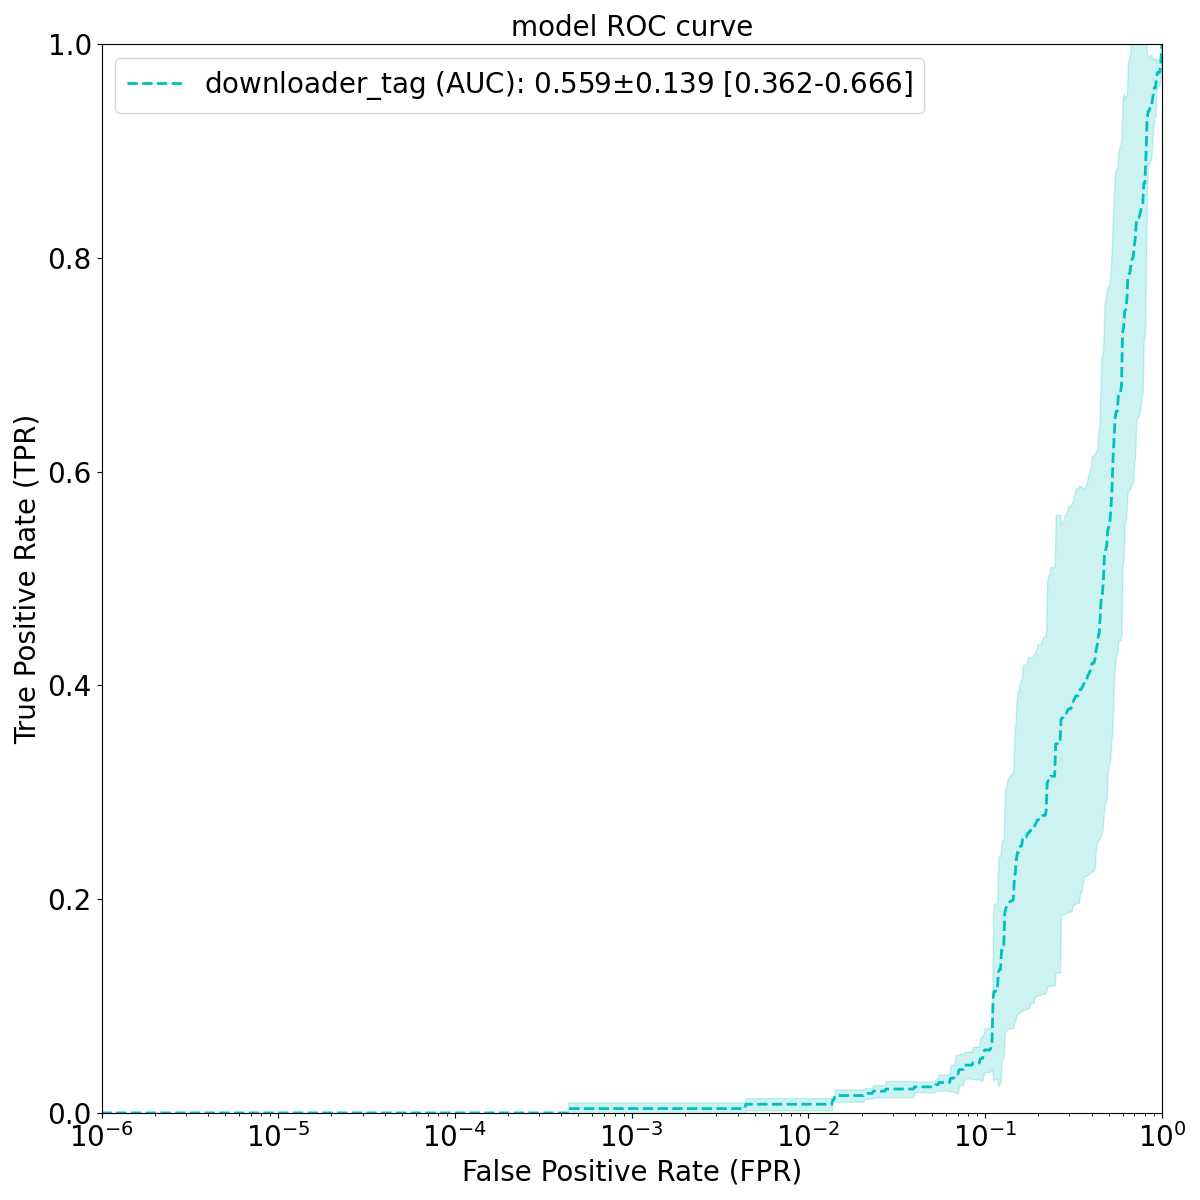
\includegraphics[width=0.6\textwidth]{./results/downloader_tag_roc_aloha.png}
        \vspace*{-0.2cm}
        \caption{ROC curve and AUC statistics of \textBF{ALOHA} model for the \textbf{Downloader Tag}. The line represents the \textit{mean} TPR at a given FPR, while the shaded region represents the \textit{standard deviation}. Statistics were computed over \textBF{3} training runs, each with random parameter initialization.}
        \label{fig:downloaderTagRocAloha}
    \end{figure}
}

\newcommand{\downloaderTagRocJointEmbedding}{
    \begin{figure}[H]
        \vspace*{-0.5cm}
        \centering
        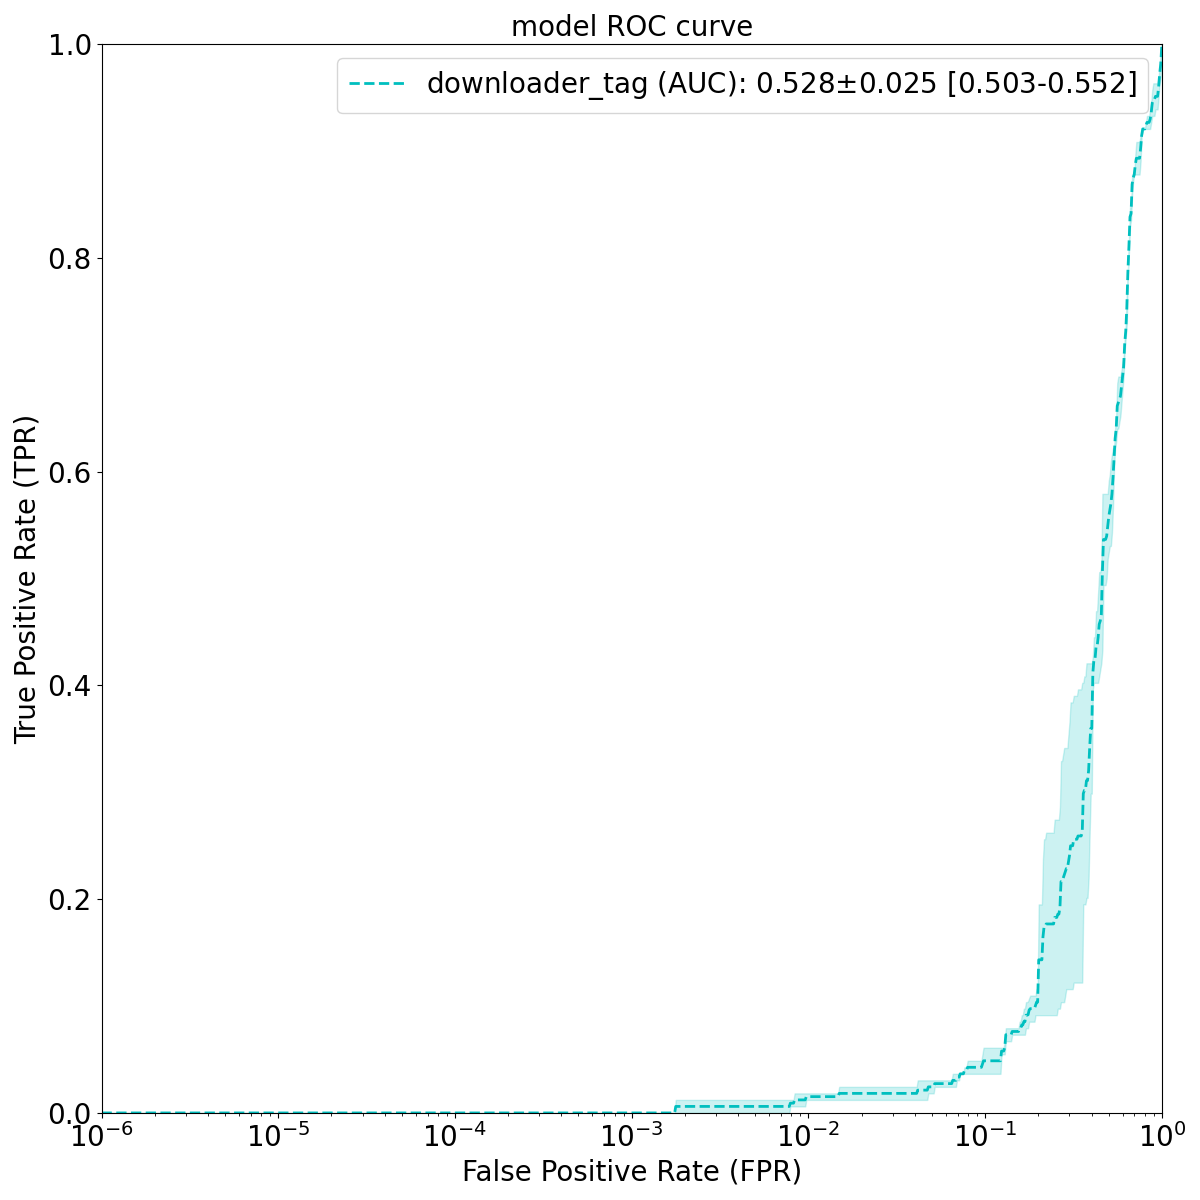
\includegraphics[width=0.6\textwidth]{./results/downloader_tag_roc_jointEmbedding.png}
        \vspace*{-0.2cm}
        \caption{ROC curve and AUC statistics of \textBF{Joint Embedding} model for the \textbf{Downloader Tag}. The line represents the \textit{mean} TPR at a given FPR, while the shaded region represents the \textit{standard deviation}. Statistics were computed over \textBF{3} training runs, each with random parameter initialization.}
        \label{fig:downloaderTagRocJointEmbedding}
    \end{figure}
}

\newcommand{\downloaderTagRocProposedMethod}{
    \begin{figure}[H]
        \vspace*{-0.5cm}
        \centering
        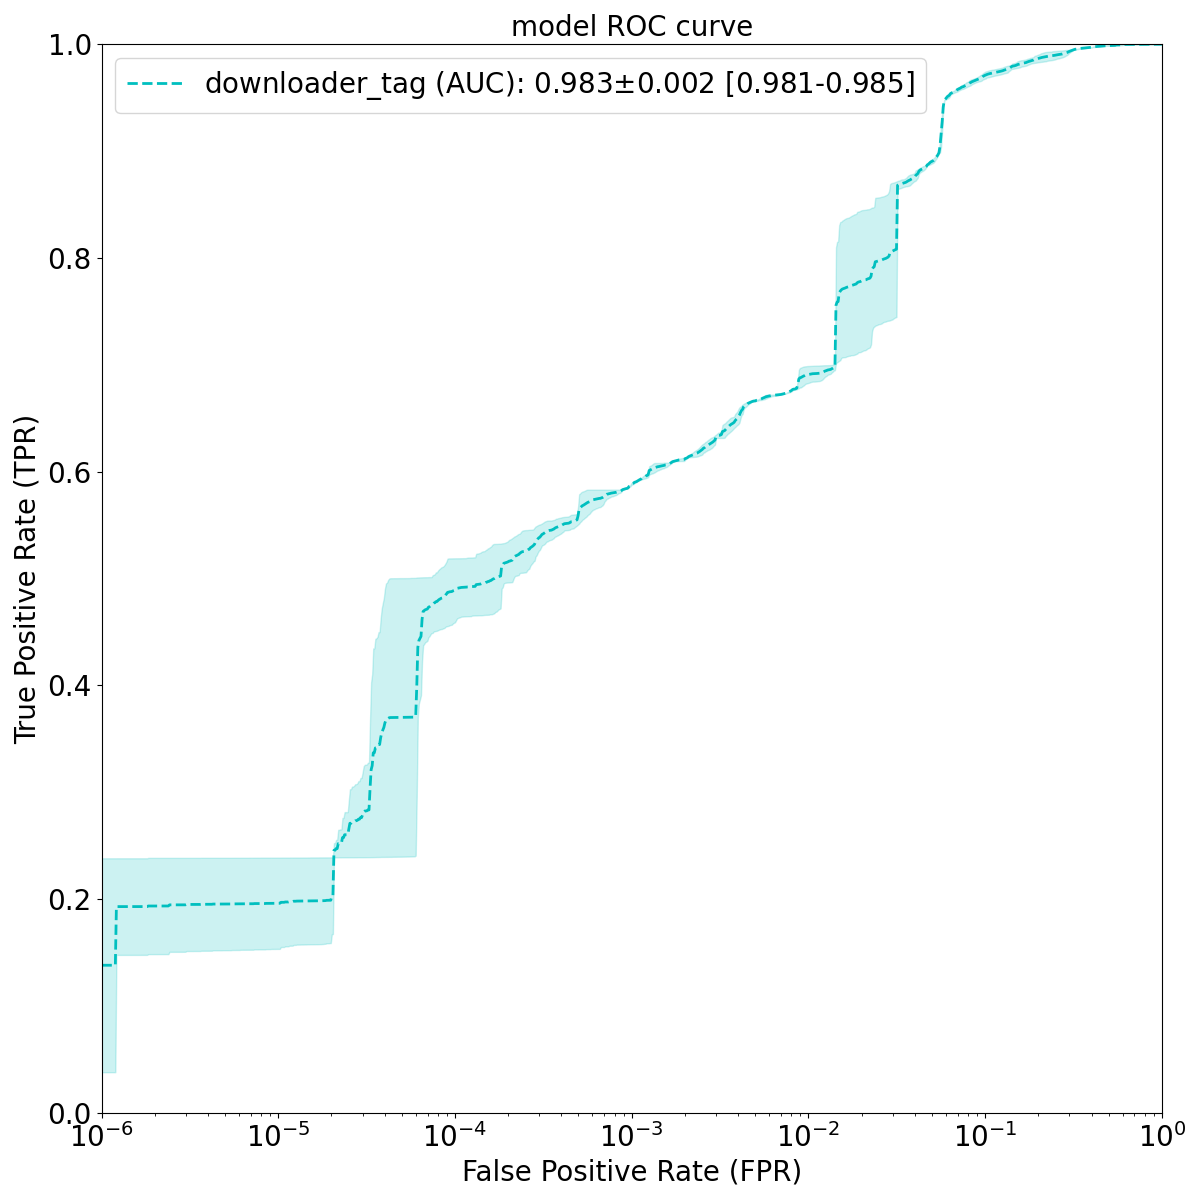
\includegraphics[width=0.6\textwidth]{./results/downloader_tag_roc_proposedModel.png}
        \vspace*{-0.2cm}
        \caption{ROC curve and AUC statistics of \textBF{Proposed Model} for the \textbf{Downloader Tag}. The line represents the \textit{mean} TPR at a given FPR, while the shaded region represents the \textit{standard deviation}. Statistics were computed over \textBF{3} training runs, each with random parameter initialization.}
        \label{fig:downloaderTagRocProposedModel}
    \end{figure}
}
